
\chapter{Project Management}

\section{Risk Assessment}

\begin{longtable}[ht]{ p{.2\textwidth} p{0.06\textwidth}  p{0.06\textwidth} p{0.06\textwidth} p{0.5\textwidth}}
  \toprule
  \textbf{Risk}
   & \textbf{Loss}
   & \textbf{Prob}
   & \textbf{Risk}
   & \textbf{Mitigation}
  %
  \\\midrule\midrule
  Laptop damaged or lost
   & 3
   & 1
   & \cellcolor{orange!50} 5
   & All work is stored using version control and periodic backups will be
  made and stored locally and in cloud storage. I have other devices that
  could be used to continue development.
  %
  \x
  Difficulty with blockchain development
   & 2
   & 3
   & \cellcolor{orange!50} 6
   & I will seek advice from my supervisor about how to tackle certain problems
  and if necessary, what aspects of my project I should change.
  %
  \x
  The application is not finished
   & 1
   & 3
   & \cellcolor{green!30} 3
   & Using agile development will ensure that I will at least have a minimal
  working application. If I feel that I am running out of time, I will focus
  on expanding test cases and improving the write-up.
  %
  \x
  No suitable large scale test environment
   & 2
   & 5
   & \cellcolor{red!40} 10
   & I do not have the infrastructure to test this project on a large network,
  however small scale tests will be possible.
  %
  \x
  Personal illness
  & 3
  & 2
  & \cellcolor{orange!50} 6
  & Depending on the amount of lost time, I may have to not complete some of the SHOULD or COULD requirements.
  \\\bottomrule\bottomrule
  \\\caption{\textit{The risk assessment of this project.}}
  \label{tab:risk assessment}
\end{longtable}

\section{Work to Date}

My work has primarily been on research, looking at how blockchain has been used to build and supplement cloud storage systems as well as how various peer-to-peer functioned and performed. 
I have proposed a design for the application to be built on the EVM. 

\begin{figure}[ht]
  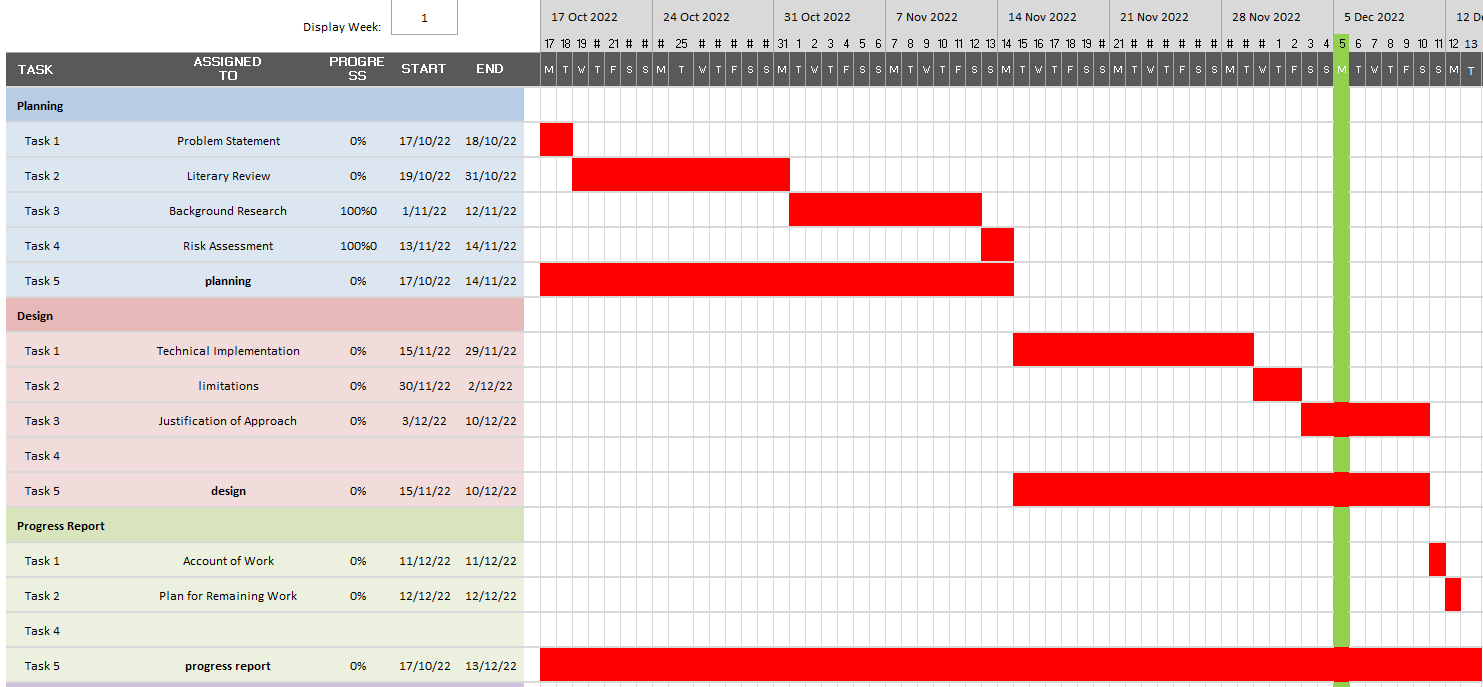
\includegraphics[width=\textwidth]{diagrams/gantt-chart-1.png}
  \caption{\textit{A Gantt chart for my work up until the progress report.}}
\end{figure}

\section{Plan of Future Work}

My project is now split into the following remaining phases:

\paragraph{Implementation \& Testing}
This phase will use agile-based, test-driven development to incrementally deliver functionally and robust pieces of code. The initial sprint will focus on the underlying architecture and provide a base system for the platform to run on, whilst later sprints will focus on improving and adding new functionality. This will also include a write-up after every sprint of what was accomplished and what wasn't.

\paragraph{Testing Strategy and Results}
This phase will be used to reflect on how test-driven development affected my project and what strategy I commonly used during development. It will also be used detail how my application fared against the tests and any problems that I am aware of with the application that I was unable to fix.

\paragraph{Evaluation}
This phase will focus on me critically evaluating the success of my project as a solution to the problem that it set out to solve. It will be used to compare it as a standalone platform and in comparison to other competitors and similar works.